\documentclass{thesis}
\usepackage{graphicx}
\graphicspath{ {./images/} }
\usepackage{color}
\usepackage{listings}
\usepackage{xcolor}

\definecolor{codegreen}{rgb}{0,0.6,0}
\definecolor{codegray}{rgb}{0.5,0.5,0.5}
\definecolor{codepurple}{rgb}{0.58,0,0.82}
\definecolor{backcolour}{rgb}{0.95,0.95,0.92}

\lstdefinestyle{codestyle}{
    backgroundcolor=\color{backcolour},   
    commentstyle=\color{codegreen},
    keywordstyle=\color{magenta},
    numberstyle=\tiny\color{codegray},
    stringstyle=\color{codepurple},
    basicstyle=\ttfamily\footnotesize,
    breakatwhitespace=false,         
    breaklines=true,                 
    captionpos=b,                    
    keepspaces=true,                 
    numbers=left,                    
    numbersep=5pt,                  
    showspaces=false,                
    showstringspaces=false,
    showtabs=false,                  
    tabsize=2
}

\lstset{style=codestyle}

\begin{document}

\pretitle{Inżynierska praca dyplomowa}
\title{Realizacja sprzętowa i programowa lidaru dwuwymiarowego}
\svnurl{https://github.com/KP191458/Lidar2d}
\author{Konrad Pławik}
\department{Wydział Fizyki Technicznej, Informatyki \par i Matematyki Stosowanej}
\promotor{dr inż. Krzysztof Lichy}
\examdate{Wrzesień 2021}
\maketitle

\newpage
\tableofcontents
\newpage

\section {Wstęp}
\subsection {Czym jest LIDAR ?}

Za wikipedią:
Lidar (od angielskiego akronimu LIDAR, utworzonego od wyrażenia: Light Detection and Ranging)
– urządzenie działające na podobnej zasadzie jak radar (Radio Detection and Ranging), ale
wykorzystujące światło lasera zamiast mikrofal. Urządzenie charakteryzuje się wysoką
rozdzielczością \cite{lidar_pl}.\\

Pierwsze użycie lasera do pomiaru odległości miało miejsce na potrzeby amerykańskiego 
wojska na początku lat 60, zaraz po wynalezieniu lasera. Było to użycie laserowego dalmierza 
model Colidar Mark II - obiekt, ze względu na swoje rozmiary, przypominał strzelbę \cite{lidar_en}.\\

Pierwsze zastosowanie urządzeń przypominających obecne Lidary to rok 1971 i działalność
Amerykańskiego Centrum Badań Fizyki Atmosfery w Boulder w Kolorado (National Center for
Atmospheric Research). Urządzenie dokonywało pomiaru wysokości chmur i zanieczyszczenia
atmosferycznego. Kolejne zastosowanie tego samego roku miało miejsce w czasie misji
Apollo 15 gdzie za pomocą sonaru laserowego (tak technologia ta była wówczas nazywana)
skanowano powierzchnię księżyca \cite{lidar_en}.\\

Ogólna zasada działania polega na połączeniu lasera z teleskopem. Laser wysyła, poprzez układ optyczny, bardzo krótkie i dokładnie wymierzone, ale silne impulsy elektromagnetyczne w widmie światła widzialnego lub podczerwonego. Na przebytym dystansie światło to ulega rozproszeniu, które jest obserwowane za pomacą teleskopu, fotodiody, fotopowielacza albo kamer CCD lub CMOS. \\

Zasadę te doskonale ilustruje rysunek z książki Paula McManamoma:
Figure 1.2 LiDAR Conceptual diagram (adapted from Ref. 3) \cite{mcmanamom}.\\
\begin{figure}[h]
    \centering
    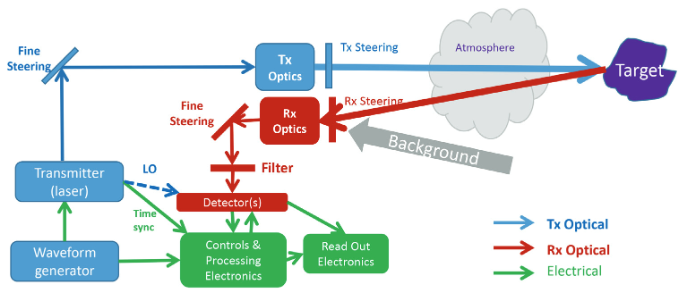
\includegraphics[scale=0.5]{lidar_concept}
    \caption{Rysunek z książki Paula McManamoma - LiDAR Conceptual diagram}
    \label{fig:lidar_concept}
\end{figure}

Dr. Pinliang Dong w swojej książce "LiDAR Remote Sensing and Applications" prezentuje wpływ zjawisk atmosferycznych na pomiary Lidaru \cite{dong}, jednak w mojej pracy pomiarów dokonywałem jedynie w pomieszczeniach zamkniętych (co z resztą sugerowała specyfikacja dalmierza TFmini Plus gdzie deklarowana przez producenta dokładność podana była dla pomieszczeń zamkniętych).\\

\subsection {Cel pracy}
Celem pracy jest zbudowanie działającej implementacji (zarówno sprzętowej jak i programowej) lidaru dwuwymiarowego za pomocą dalmierza laserowego oraz silnika krokowego. Te dwa urządzenia będą rdzeniem implementacji która za pośrednictwem mikrokontrolera będzie w stanie przekazać do komputera dane z których napisany przez nas program wygeneruje dwuwymiarowy obraz pomieszczenia.

\subsection {Współczesne zastosowanie lidarów}
Lidary mają dzisiaj szerokie zastosowanie: zarówno cywilne jak militarne. Technologia ta ma zastosowanie w architekturze, budownictwie, meteorologii, wywiadzie wojskowym i cywilnym, przemyśle produkcyjnym, na kolei czy w kartografii.\\

Pomimo że moja praca skupia się na podstawach działania i jest implementacją czysto amatorską, pragnąłbym przybliżyć nieco lepiej współczesne zastosowanie zaawansowanych technologicznie lidarów. Pozwoli to zrozumieć czemu technologia ta jest dziś tak ważna i dlaczego stanowi tak istotny element rozwoju wielu gałęzi gospodarki.\\

\subsubsection{Zastosowanie na kolei}
Ciekawym przypadkiem użycia lidarów jest zastosowanie przy inwentaryzacji i inspekcji torów kolejowym. Urządzenie skanujące umieszczone jest na frontowej części pociagu i dokonuje ciągłego skanowania zarówno torów, terenu jak i pozostałych elementów infrastruktury kolejowej (słupów, peronów, barierek a nawet całych stacji).\\

\begin{figure}[h]
    \centering
    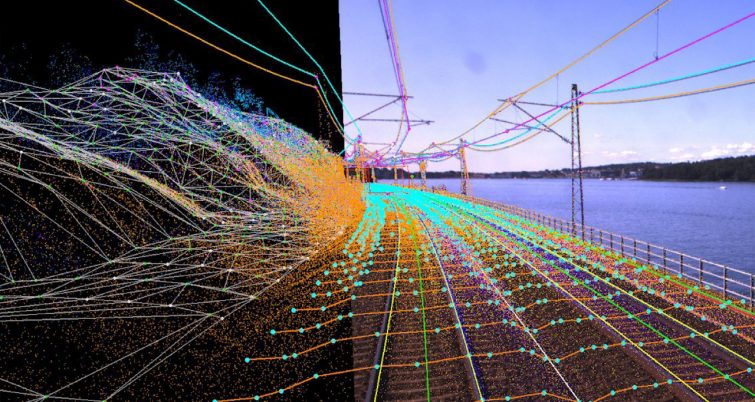
\includegraphics[scale=0.7]{LiDAR-AC-Image-1-755x402}
    \caption{Przykład skanu z artykułu: \cite{tory}}
    \label{fig:tory}
\end{figure}

Dzięki cyklicznym pomiarom i porównywaniu wyników system jest z stanie znaleźć nawet najdrobniejsze zmiany w terenie czy infrastrukturze. Pozwala to przewidzieć osiadanie terenu, odkształcenia torów czy uszkodzenia infrastruktury zanim jeszcze zmiany te okażą się krytyczne i staną się powodem usterek. Co więcej system jest w stanie przewidzieć np. optymalną prędkość (konfortową dla pasażerów) bądź uprzedać o istotnych niebezpiecznych zakrętach. System z powodzeniem stosowany w Wielkiej Brytanii, Francji czy Indiach.\\

Z laserowej inspekcji torów korzysta również nowojorskie metro.

\subsubsection{Zastosowanie w budownictwie}
Zastosowanie w budownictwie jest bardzo szerokie natomiast kilka ciekawych rozwiązań posiada w swojej ofercie firma Leica. Serię BLK nazwałbym kamieniami milowymi współczesnego rozwoju technologii Lidar.\\

\textbf{BLK360}

\begin{figure}[h]
    \centering
    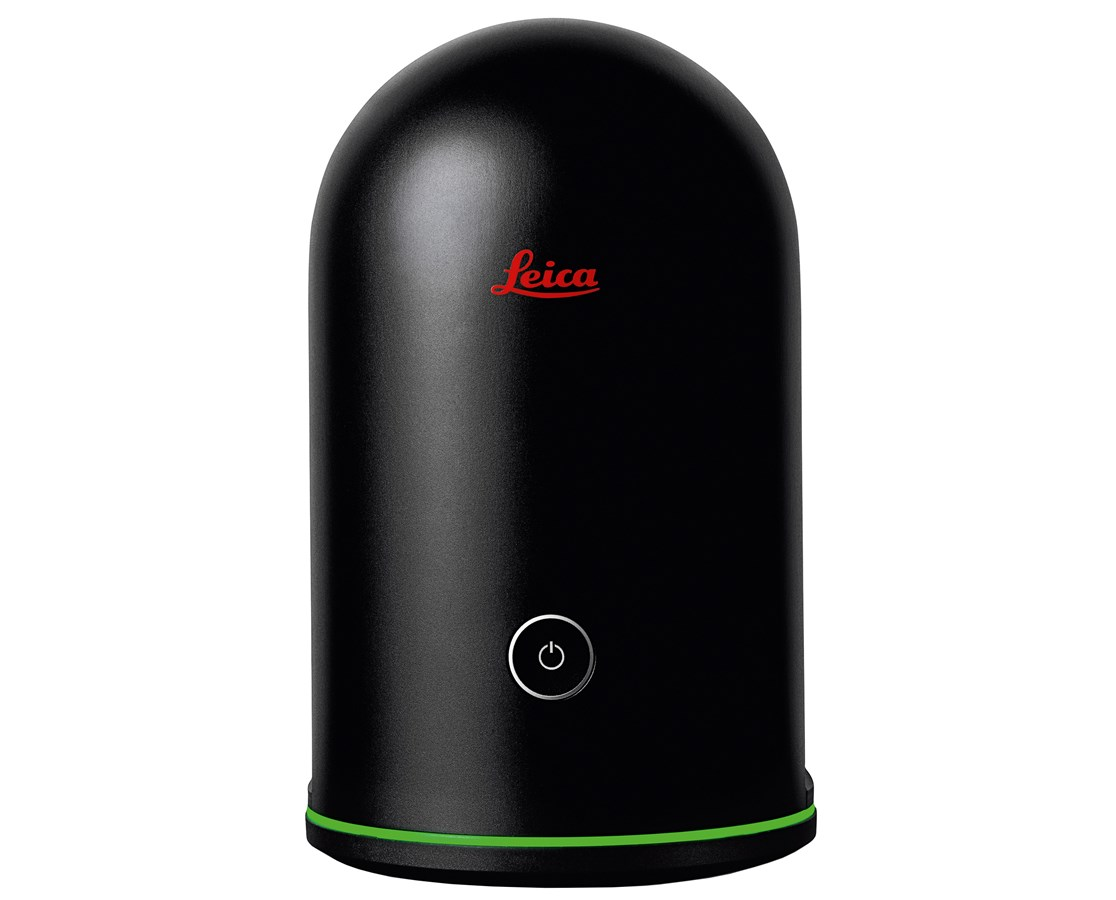
\includegraphics[scale=0.2]{Leica_BLK360_Front2}
    \caption{Frontowy panel urządzenia BLK360 \cite{blk360}}
    \label{fig:blk360}
\end{figure}

Urządzenie jest urządzniem statycznym. Zczytuje 360,000 punktów na sekundę z milimetrową dokładnością. Zasięg do 60 metrów. Dodatkowo rejestruje obraz z 3 kamer dzięki czemu możliwe jest również zastosowanie sztucznej inteligencji (głównie technologii \textbf{Uczenia Maszynowego}) do rozpoznawania obiektów w budynku (okna, drzwi, instalacje) i tworzenia interaktywnego modelu \textbf{BIM (Building Information Modeling)}.\\

\textbf{BLK2GO}

Mobilna i ulepszona wersja BLK360. Pozwala tworzyć modele całych budynków w czasie rzeczywistym. Dodatkowo również obsługuje rozpoznawanie elementów budynku i tworzy model BIM.\\
\begin{figure}[h]
    \centering
    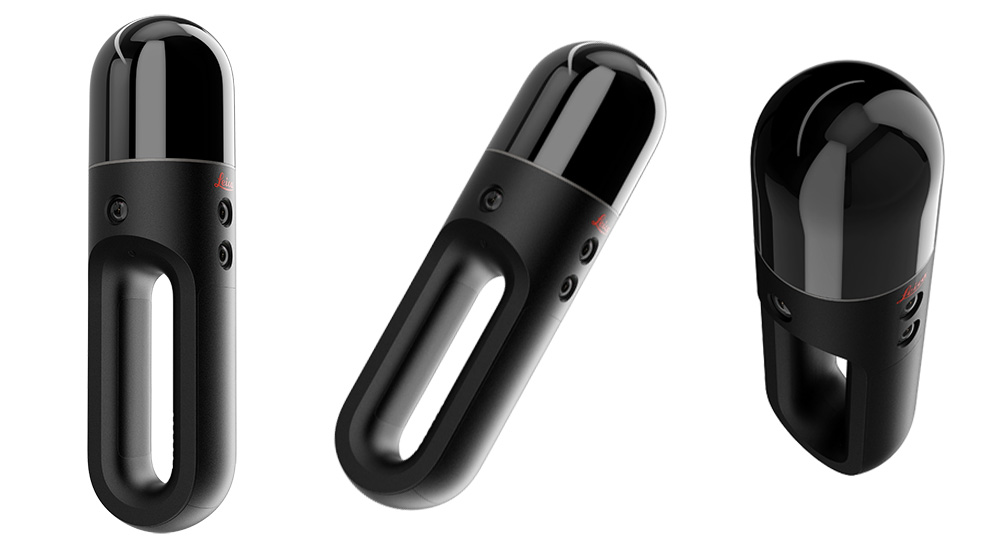
\includegraphics[scale=0.4]{blk2go}
    \caption{Frontowy panel urządzenia BLK2GO \cite{blk2go}}
    \label{fig:blk2go}
\end{figure}

\textbf{BLK2FLY}

\begin{figure}[h]
    \centering
    \includegraphics[scale=0.4]{blk2fly}
    \caption{Render planowanego wyglądu urządzenia BLK2FLY \cite{blk2fly}}
    \label{fig:blk2fly}
\end{figure}

We wrześniu 2021 roku pojawił się oficjalny komunikat firmy Leica dotyczący kolejnego projektu - \textbf{BLK2FLY}. Urządzenie wykorzystuje drona i jest w pełni autonomiczne. Użytkownik, na urządzeniu mobilnym, wybiera jedynie porządany obiekt (np. cały budynek) a automatycznie sterowany drone samodzielnie dokonuje wszyskich zadanych pomiarów. Ogromna mobilność drona pozwala na pomiar trudno dostępnych dla człowieka miejsc.\\

\textbf{BLK247}\\
System monitoringu przemysłowego który prócz technologii Lidar wykorzystuje jeszcze obraz wideo i pomiar temperatury powierzchni.\\
\begin{figure}[h]
    \centering
    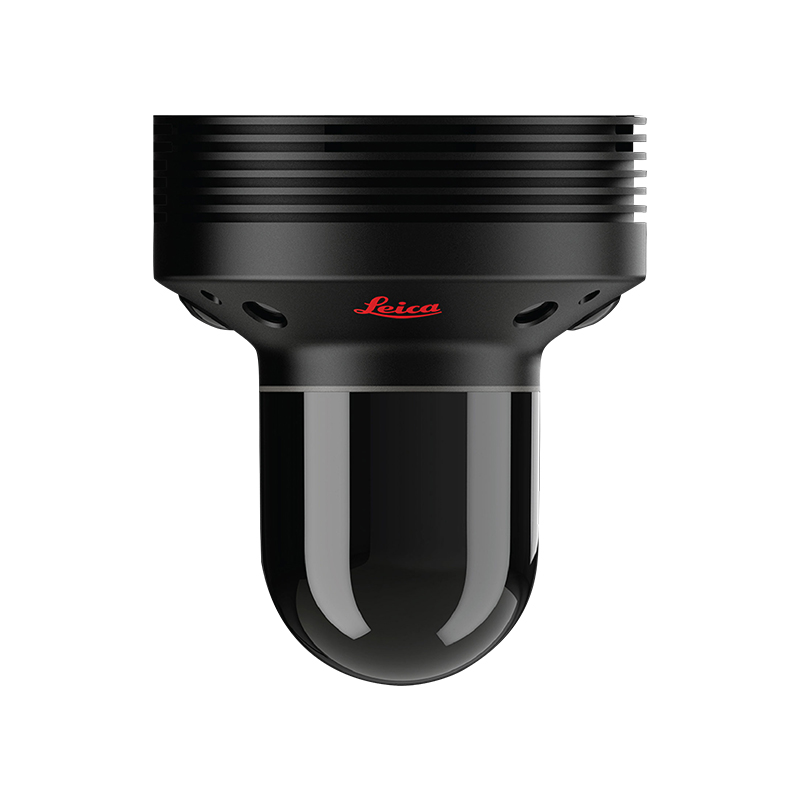
\includegraphics[scale=0.3]{BLK247}
    \caption{Pojedyncza kamera systemu BLK247 \cite{blk247}}
    \label{fig:blk247}
\end{figure}
Przewagę nad systemami monitoringu wykorzystującymi jedynie kamery jest taka że system jest w stanie tworzyć obraz i wykrywać ruch nawet przy całkowitej ciemności. Dodatkowo system termowizyjny wykrywa ludzi i zwierzęta a technologie AI pozwalają klasyfikować wykrywane obiekty.

\begin{figure}[h]
    \centering
    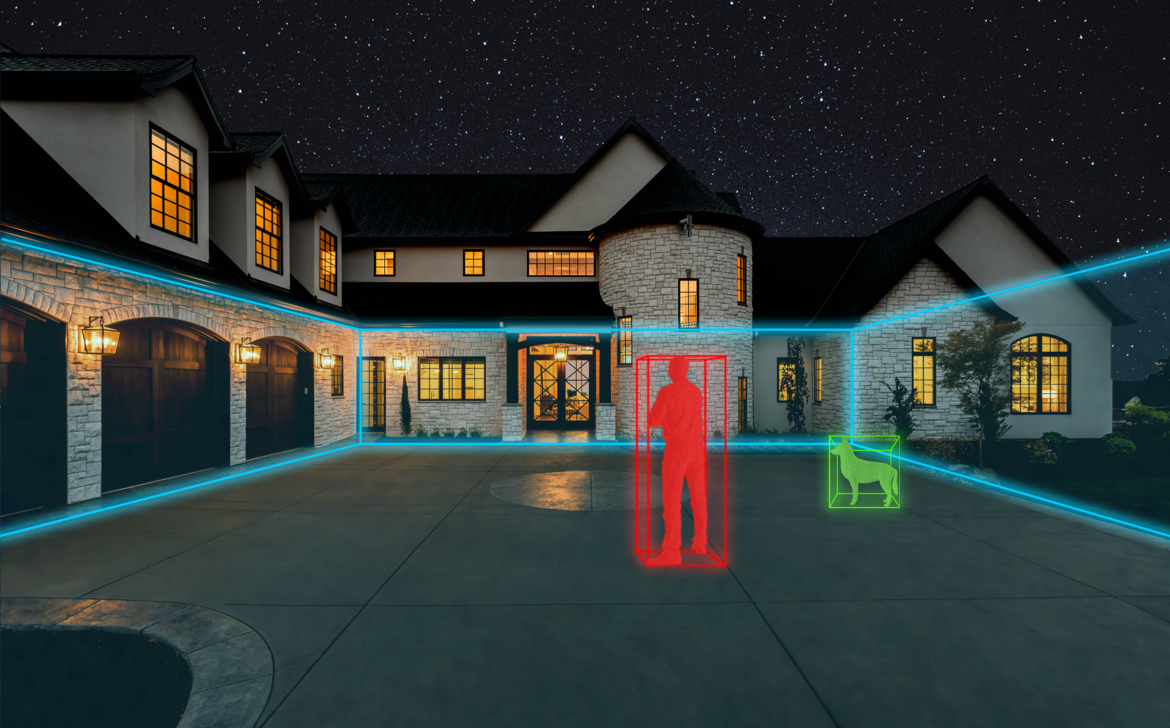
\includegraphics[scale=0.3]{BLK247-house-night_0}
    \caption{Poglądowy schemat działania ze strony internetowej producenta \cite{blk247}}
    \label{fig:house-night}
\end{figure}

\newpage
\subsubsection{Zastosowanie w kartografii}
Jednym z pierwszych zastosowań lidarów było zastosowanie ich w kartografii. Dzisiaj zastosowanie to jest szeroko stosowane zarówno przez wojskowe agencje wywiadowcze jak i korporacje jak Google czy Apple dla swoich aplikacji służących do nawigacji w terenie.\\


\section {Zasada działania}

\subsection {Jak powstaje obraz}

Opracowana przeze mnie implementacja opiera się o pomiar odległości dalmierza od elementów pomieszczcenia dla każdej z możliwości położenia silnika. Innymi słowy silnik obraca się w okół własnej osi a wraz z każdym krokiem wykonuje pomiar odległości.\\

\begin{figure}[h]
    \centering
    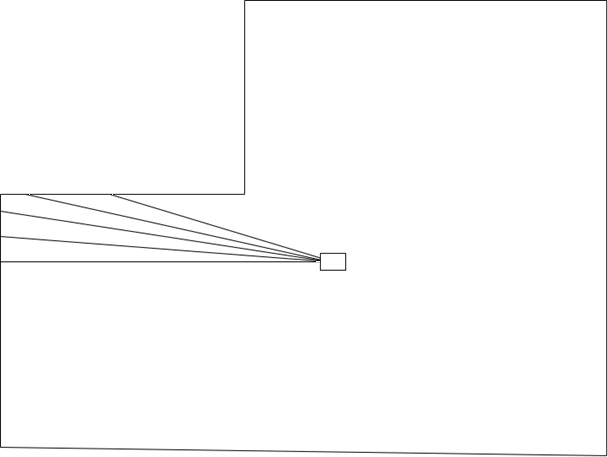
\includegraphics[scale=0.4]{how_it_works_01}
    \caption{Dalmierz na silniku krokowym wykonuje pomiary co jeden krok}
    \label{fig:how_it_works_01}
\end{figure}

Następnie pomierzona odległość zostaje wymnożona przez sinus i cosinus kąta wyznaczonego przez kolejne kroki. Obliczenia te pozwolą nam wyznaczyć wspólrzędne kartezjanskie każdego z mierzonych punktów. Dodać należy że pełny obrót silnika ma 400 gradów, dokonuje więc przeliczenia konta na wartość radianową.\\

\begin{figure}[h]
    \centering
    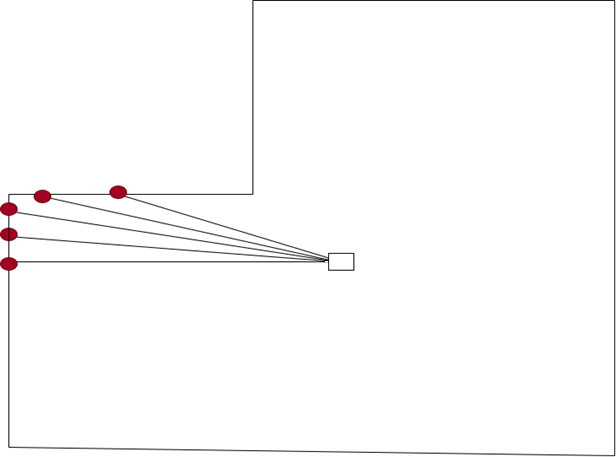
\includegraphics[scale=0.4]{how_it_works_02}
    \caption{Wyznaczane są współrzędne kartezjańskie każdego z punktów}
    \label{fig:how_it_works_02}
\end{figure}

Pełny cykl obrotu silnika daje nam przyblizony obraz całego wewnętrznego obrysu pomieszczenia.\\

\begin{figure}[h]
    \centering
    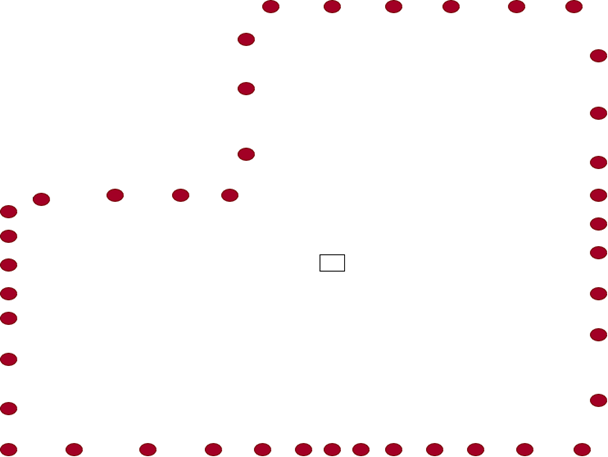
\includegraphics[scale=0.4]{how_it_works_03}
    \caption{Wszystkie wyznaczone punkty dają obrys pomieszczcenia}
    \label{fig:how_it_works_03}
\end{figure}

Na dokładność obrazu składaja się: dokładność pomiaru odległości wykonana przez dalmierz, dokładność kąta obrotu silnika krokowego, dokładność obliczeń dla środowiska w którym napisany jest program (Python).\\

Niepewności dla każdego z urządzeń wyznaczone zostały w rodziale poświęconym specyfikacji strzętowej projektu.\\
\section {Implementacja sprzętowa}
\subsection {Wykaz urządzeń}

W implementacji wykorzystane zostały następujące urządzenia:

\begin{enumerate}
\item Dalmierz Laserowy TFMini Plus UART/I2C
\item Silnik Krokowy 42HM48-1206 400 kroków
\item Arduino Uno
\item Sterownik A4988 model: STSPIN220
\item Zasilacz Laboratoryjny Zhaoxin RXN-305D
\item Zestaw przewodów
\item Płytka stykowa
\item Metalowe uchwyty dalmierza
\item Libela poziomicy
\end{enumerate}

\subsection {Specyfikacje urządzeń}
Implementacja wymagała zakupu i podłączenia ze sobą kilku urządzeń. Niektóre z nich zostały dobrane pod kątem wyjątkowych parametrów, inne były jedynymi z wielu spełniających wymagania projektowe. Poniżej zebrałem najistotniejsze argumenmty za wyborem tych właśnie urządzeń.\\

\textbf{Dalmierz Laserowy TFMini Plus UART/I2C}\\
Dalmierz laserowy działający dla ogległości od 0.1 do 12 metrów. Dokładność wynosi 5 cm (więcej w rozdziale o nepewnościach pomiarowych). Zasilany napięciem 5V. Komunikacja możliwa prze UART oraz I2C. Długość fali 850 nm. Częstotliwość pracy: od 1 Hz do 1000 Hz. Wymiary: 35 x 21 x 18,5 mm. Masa: 11 g.\\

\textbf{Silnik Krokowy 42HM48-1206}\\
Silnik wybrany ze względy na wysoką rozdzielczość - 400 kroków przy pełnym obrocie. Wadą był niski prąd zasilania (4.0V) co zawięziło wybór modelu sterownika.  Unipolarny, sześcio przewodowy. Pobiera prąd 1200 mA na cewkę. Moment wynosi 3,17 kg*cm (0,31 Nm). Wymiary to 42 x 42 x 48 mm (NEMA 17).\\

\textbf{Arduino Uno}\\
Arduino Uno Rev3 - Uniwersalny moduł od Arduino Uno z mikrokontrolerem AVR ATmega328. Posiada 32 kB pamięci Flash, 2 kB RAM, 14 cyfrowych wejść/wyjść, 6 wejść analogowych oraz popularne interfejsy komunikacyjne. Wykorzystałem w projekcie ze względy na prostą obsługę, wysoką dostępność bibliotek oraz doświadczenia zdobyte podczas studiów.\\

\textbf{Sterownik A4988 model: STSPIN220}\\
Strerownik na bazie popularnego chipsetu A4988. Model wybrany ze względu na współpracę w silnikami niskoprądowymi (4.0 V).\\

Schemat:\\
\begin{figure}[h]
    \centering
    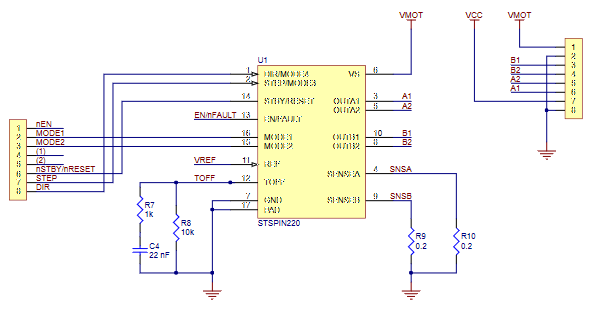
\includegraphics[scale=0.6]{a4988_scheme}
    \caption{Schemat modelu STSPIN220}
    \label{fig:a4988_scheme}
\end{figure}

\textbf{Zasilacz Laboratoryjny Zhaoxin RXN-305D}\\
\\

\textbf{Zestaw przewodów}\\
\\

\textbf{Metalowe uchwyty dalmierza}\\
\\

\textbf{Libelae poziomicy}\\
\\

\subsection {Niepewności pomiarowe}
Każde z wykorzystanych urządzeń posiada pewną niepewność mierzowych i wskazywanych przez siebie wartości. Należy mieć na uwadze te niepewności oraz fakt że jeśli wykorzsytujemy naraz kilka różnych odczytów to niepewności nałorzą się na siebie.\\

\textbf{Niepewność dalmierza laserowego TFMini Plus}\\
Według specyfikacji dostarczonej przez producenta pokładność pomiarów dla odległości pomiędzy 0.1-6 metrów wynosi $\pm$ 5cm a dla odległości 6-12 metrów to $\pm$ 1\%.\\

\textbf{Niepewność silnika Krokowego 42HM48-1206}\\
Specyfikacja producenta nie podawała żadnej wartości niepewności kąta obrotu silnika.\\

\textbf{Niepewność Arduino Uno}\\
W implementacji wykorzystaliśmy jedynie cyfrowe interfejsy modułu Arduino. Nie ma więc obaw o niedokładność taką jak generują interfejsy analogowe urządzenia.\\

\textbf{Niepewność sterownika A4988 model: STSPIN220}\\
Specyfikacja producenta nie podaje dokładności sterownika, natomiast znaleziona w intenecie literatura \cite{microstepping} dla pojedynczego kroku na obrót podaje dokładność 100 \% (dla połowy kroku 70.71 \% a dla ćwiartki 38.27 \%). Dla większości badancyh przypadków użyto jednego kroku na obrót więc niepewność przyjmuję równą zero.\\

\textbf{Niepewność zasilacza Laboratoryjnego Zhaoxin RXN-305D}\\
Producent deklaruje dokładność wskazań zarówno woltomierza jak i amperomierza na poziomie 1\% + 1 cyfra znacząca.\\

\textbf{Niepewność przewodów}\\
Specyfikacja podaje jedynie 4. kategorię przetestowania.\\

\textbf{Niepewność uchwytów dalmierza}\\
Możliwe do zmierzenia wymiary w czasie wykonania przeze mnie elementu zmierzone zostały suwmiarką o dokłądności 0.1mm.\\

\textbf{Niepewność libeli poziomicy}\\
Produkcja austriacka. Brak danych o dokładności.\\
\section {Implementacja programowa}

\subsection {Użyte języki programowania i biblioteki}
Implementacja składała się z dwóch programów: Pierwszy z nich został napisany w jezyku programowania dla mikrokontrolerów Arduino (opartym na środowisku Wiring i zasadniczo na języku C/C++ \cite{arduino}) i służył do odczytu danych z dalmierza oraz sterowania silnikiem. Drugi został napisany w języku Python w wersji 3.9.5. i służył do generowania obrazu z odczytanych wcześniej punktów.\\

W programie napisanym w środowisku Arduino wykorzystaliśmy biblioteki:

\begin{enumerate}
    \item \textbf{AccelStepper 1.61.0} - biblioteka do sterowania silnikiem.
    \item \textbf{TFMini 1.01} - bilioteka do odczytu danych z dalmierzy serii TF.
\end{enumerate}

Napisany w języku Python program do generowania obrazu z przekazanych punktów wykorzystuje następujące biblioteki:

\begin{enumerate}
    \item \textbf{PyQt5}
    \item \textbf{pyqtgraph}
    \item \textbf{pyserial}
\end{enumerate}

Dwie pierwsze to biblioteka Qt służąca do budowy interfejsów graficznych i jej moduł do wykresów. Ostatnia to biblioteka do odczytu danych z portów szeregowych Arduino.\\

W pierwotnej koncepcji oba programy miały być napisane w języku C++. Problemem okazało się nieprzystosowanie najpopularniejszych bibliotek (m.in. gnuplot) do pracy z dynamicznymi danymi. Kolejna koncepcja poddawała pod rozwagę użycie czysto obiektowych języków Java bądź C\#. Ze względu na dynamiczny charakter pracy urządzenia i istotną dla niego wysoką szybkość przesyłu danych z dalmierza istniało podejrzenie że Java może mieć problem z rysowaniem tak dużej ilości wykresów w tak któtkim czasie. Implementacje rysowania wykresów dynamicznych pod swoją powłoką rysowały dla nowych danych kolejny raz cały wykres i podmieniały wygenerowany rysunek.\\

Optymalny okazał się język Python. Użyta biblioteka również rysowała za każdym razem cały wykres od nowa ale jej optymalizacja umożliwiała płynną obsługę napływających danych. Język Python ma również wbudowane funkcje parsowania tekstu i prostą obsługę tablic.

\subsection {Podstawy prawne użytego oprogramowania}
Arduino korzysta z licencji \textbf{LGPL} \cite{arduino_lic}, a użyte przeze mnie biblioteki
AccelStepper z \textbf{GPL} \cite{accelstepper_lic} a TFMini z \textbf{Public Domain} \cite{tfmini_lic}.\\

Python rozwijany jest jako projekt Open Source zarządzany przez Python Software Foundation, która jest organizacją non-profit. Jest udostępniony na licencji kompatybilnej z \textbf{GPL} \cite{python_lic}. PyQt5 jest na licencji \textbf{GPL v3.} \cite{pyqt5_lic}. PyQtGraph jest na licencji \textbf{MIT open-source license}. \cite{pyqtgraph_lic}\\

Niniejsza praca nie jest wykorzystaniem komercyjnym więc żadna z licencji nie zastała naruszona.

\subsection {Analiza wybranych fragmentów kodu}

Poniżej analiza najważniejszych elementów kodu źrodłowego które złożyły się na implementacje od strony oprogramowania.\\

\textbf{Odczyt danych z dalmierza}

\begin{lstlisting}[language=C++, caption=Odczyt danych z dalmierza]
    void loop() { 
        if (Serial1.available()) {  //check if serial port has data input
          if(Serial1.read() == HEADER) {  //assess data package frame header 0x59
            uart[0]=HEADER;
            if (Serial1.read() == HEADER) { //assess data package frame header 0x59
              uart[1] = HEADER;
              for (i = 2; i < 9; i++) { //save data in array
                uart[i] = Serial1.read();
              }
              check = uart[0] + uart[1] + uart[2] + uart[3] + uart[4] + uart[5] + uart[6] + uart[7];
              if (uart[8] == (check & 0xff)){ //verify the received data as per protocol
                dist = uart[2] + uart[3] * 256;     //calculate distance value
                strength = uart[4] + uart[5] * 256; //calculate signal strength value
                temprature = uart[6] + uart[7] *256;//calculate chip temprature
                temprature = temprature/8 - 256;
                Serial.print(step);
                Serial.print(" ");
                Serial.print("dist = ");
                Serial.print(dist); //output measure distance value of LiDAR
                Serial.print('\t');
                Serial.print("strength = ");
                Serial.print(strength); //output signal strength value
                Serial.print("\t Chip Temprature = ");
                Serial.print(temprature);
                Serial.println(" celcius degree"); //output chip temperature of Lidar
                take_step();         
              }
            }
          }
        }
      }
\end{lstlisting}
Powyższy kod jest kopią kodu z przykladów z biblioteki urządzeń TFMini. Kod działa w pętli ciągłej. Kod sprawdza odczytany na początku nagłówek z danych z portu. Jeśli nagłówek jest prawidłowy odczytane dalej wartość są umieszczane w tablicy typu int. Kolejnym krokiem jest konwersja odczytanych danych na porządane typy i przypisanie ich do zmiennych (zmienne oraz ich nazwy zostały zainicjowane wcześniej). Następnym krokiem jest wypisanie odczytanych danych na port wyjściowy urządzenia. Implementacja została uzupełniona o ostatni krok wywołanie funkcji take\_step() która obraca silnik krokowy o kolejny krok. Kod fukcji został opisany poniżej.\\

\textbf{Przesunięcie osi silnika o kolejny krok}

\begin{lstlisting}[language=C++, caption=Przesunięcie o kolejny krok]
void take_step(){
  if(dir==0)
    step++;
  else
    step--;

  if(step==0)
    dir=0;
  if(step==400)
    dir=1;

  myStepper.moveTo(step);
  delay(100);
  myStepper.run();
}
\end{lstlisting}
Funkcja zawiera proste instrukcje warunkowe które sprawdzają który krok został ostatnio podjęty (według zainicjowanego globalnie licznika kroków) oraz kierunek przesuwu. Przesów silnika odbywa się za pomocą rekomendowanej dla silnika biblioteki. Funkcja ta umożliwiła optymalny - wahadłowy - ruch osi silnika.\\

\textbf{Rysowanie punktów obrazu}

\begin{lstlisting}[language=Python, caption=Rysowanie obrazu]
    def update_plot_data(self):

        m = [ser.readline(100).decode('utf-8')]
        n = m[0].split()
        print(n)
        i = int(n[0])
        x_value = float(int(n[3])*math.sin(int(n[0])*math.pi/200.0))
        y_value = float(int(n[3])*math.cos(int(n[0])*math.pi/200.0))

        self.x.pop(i)
        self.x.insert(i, -x_value)

        self.y.pop(i)
        self.y.insert(i, y_value)

        self.data_line.setData(self.x, self.y)  # Update the data.
\end{lstlisting}

Funkcja ta odczytuje dane z portu szeregowego Arduino (całe linijki tekstu) a następnie dane umieszcza w tablicy danych typu string (funkcja split()). Natępnie używamy z tej tabeli jedynie aktualnego kąt (w gradach) i odległości (odczytanej z dalmierza). Dane te umożliwiają wylicznie współrzędnych rysowanych punktów (x\_value i y\_value). Kolejno punkty te zostają wrzucone w odpowiednie miejsca w kontener pozostałych punktów a na koniec obraz zostaje ponownie wygenerowany w celu aktualizacji o odczytany punkt.
\section {Eksperymenty}
\subsection {Experyment pierwszy: pomieszczenie codziennego użytku}
Pierwszy z wykonanych eksperymentów polegał na wygenerowaniu obrazu pomieszczenia w którym pracowałem nad pisaną właśnie pracą dyplomową (salon z aneksem kuchennym).
Pomieszczenie ma XX metrów kwadratowych i znajdują się w nim elementy codziennego użytku - lodówka, zlew kuchenny, kwiaty na parapecie oraz otwór dzwiowy łączcy pomieszczenie z przedpokojem. Wymiary pokoju to XX m x XX m.\\


Dla opisanego pomieszczenia wygenerowany został następujący obraz:
\begin{figure}[h]
    \centering
    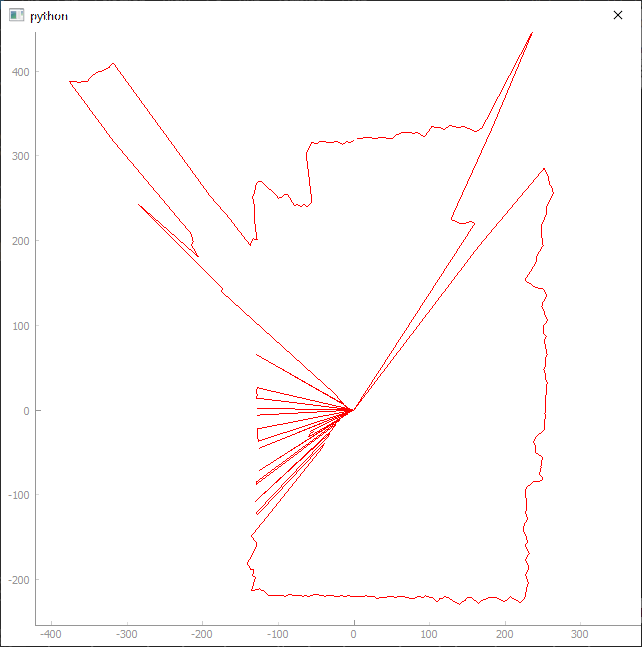
\includegraphics[scale=0.5]{experiment_1_plot}
    \caption{Wygenerowany obraz pomieszczenia - salonu z aneksem kuchennym}
    \label{fig:experiment_1_plot}
\end{figure}

W chwili generowania obrazu dalmierz znajdował się ok. 110 cm ponad powierzchnią podłogi, dzięki czemu nie znalazły się na nim stojące w pokoju umeblowanie.

\subsection {Experyment pierwszy: analiza wygenerowanego obrazu}

Wygenerowany obraz przedstawia dosyć wierne odwzorowanie badanego pomieszczenia. Ze względu na amatorski charakter urządzenia znalazło się w nim jednak kilka przekłamań:

\begin{enumerate}
    \item Otwór dzwiowy spowodował odczyt odległości do ściany w sąsiednim pomieszczeniu (przedpokoju) oraz kolejnym pokoju.
    \item Połyskująca powierzchnia lodówki wprodziła przekłamanie na jej frontowej powierzchni - wygenerowany jej obraz sprawia mylne wrażenie rombu. 
    \item Metalowy kran o obłym krztałcie prowadza kilka znieszkałceń - ze względu na refleksję promienia lasera.
    \item Na parapecie stoją doniczki z kwiatami co uwzględnione zostało na neregularnych kształtach wykresu
    \item Puste ściany z kąty proste odzwierciedlone zostały w dosyć dużą dokładnością.
    \item Ściana na przeciw okna została odzwierciedlola z kilkoma przekłananiami (odczyty zerowych wartości dalmierza). Powierzchnia w tym miejscu nie różni się niczym od pozostałch powierzni, zarówno użytą farbą, kolorem jak i nasłonecznieniem. Przyczyna błędnych wskazań w tym miejscu pozostaje nieznana.
\end{enumerate}

\newpage
\subsection {Experyment drugi: ocena użytej rodzielczości}

W drugim eksperymencie chciałem przekonać się o dokładności dalmierza i o tym czy zastosowana przez mnie rodzielczość (400 króków na pełen obrót) jest wystarczająca.\\

W tym celu wyłączyłem zasilanie silnika krokowego, przez co dalmierz zczytywał wciąż tę samą ogległość. Program jednak nadawał sygnał do zmiany kąta przez co przekonany był o obrocie silnika. W skutek tego otrzymaliśmy obraz okręgu (ta sama odległość dla "każdego" z kątów).

\begin{figure}[h]
    \centering
    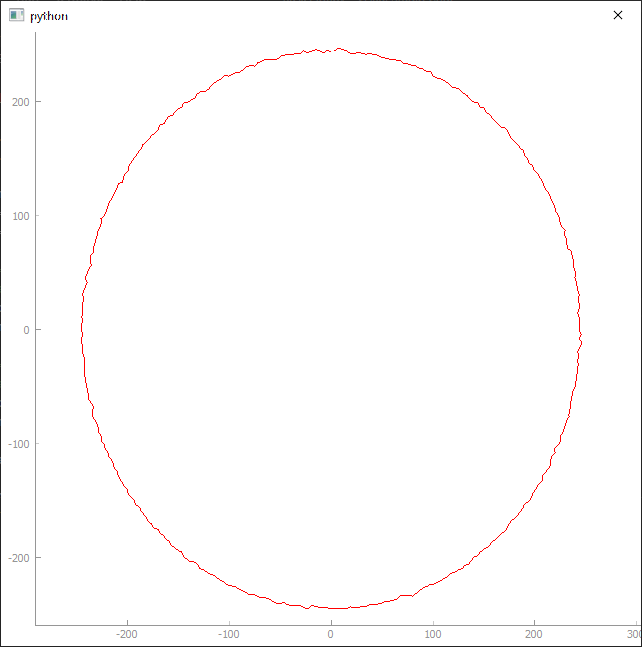
\includegraphics[scale=0.5]{experiment_2_plot}
    \caption{“Time is a flat circle” Friedrich Nietzsche}
    \label{fig:experiment_2_plot}
\end{figure}

\subsection {Experyment drugi: analiza wygenerowanego obrazu}

Wahania odczytów dalmierza różniły się od siebie z reguły o 1-2 cm, czasem o 3 cm. Wartość ta mieści się w podawanym w specyfikacji producenta zakresie.\\

Ilość wygenerowanych punktów (400) pozwoliła odzrować okrąd z bardzo dużą dokładnością. Krzywizna okręgu jest gładka a jej krztałt nie jest sprawia wrażenia widocznych pixeli (prostych linii wynikających ze zbyt rzadkiej siatki punktów). Nie ma potrzeby zwiększania rozdzielczości pracy urządzenia.\\

\section {Napotkane problemy}
\subsection {Synchronizacja odczytu danych z dalmierza}
Pierwotnym założeniem było aby ruch silnika krokowego był funkcją nadrzędną a odczyt odległości z dalmierza odbywał się tak jak nakazuje kod sterujący obrotem silnika. W takiej implementacji ok 70 \% odczytów odległości dawała puste odczyty. Zastosowanie opóżnienia nie przynosiło poprawy. Prostym rozwiązaniem okazało się uzależnienie obrotu silnika od odczytu odległości - innymi słowy: dopiero gdy odczytaliśmy pomiar ogledłości z dalmierza nadawaliśmy do silnika sygnał przemieszczenia o kolejny krok (z zastosowaniem dla pewności niewielkiego opóźnienia).\\

Najistotniejszym skutkiem uzależnienia przesówu silnika od odczytu dalmierza był brak możliwości dokładnego wysterowania prędkością obrotu silnika. Jedyna możliwość to zastosowanie dłuższego opóźnienia co skutkowało tym że czas wykonania pełnego obrotu urządzenia mogliśmy jedynie wydłużyć. 

\subsection {Refleksyjne powierzchnie}
Nawet lekki połysk powierzchni (np. kran czy lodówka) wprowadzały duże rozbierzności pomiędzy mierzoną a faktyczną odległością. W przypadku większego stopnia refleksyjności i nieregularnych krztałtów - jak np. wyżej wspomniany kran kuchenny - musiałem uciec się do prób okrycia jego powierzchni materiałami o nierefleksyjnej powierzchni.

\subsection {Okna}
Okna były kolejnym problematycznym elementem analizowanych pomieszczeń. Refleksyjna powierzchnia szyb dawała odczyty przekłamane w porównianiu z prawdziwą odległością. Co więcej elementy za oknem były niekiedy daleko poza zakresem w jakich pracuje dalmierz (12 metrów).\\

Skutkiem istnienia okien w badanych pomieszczeniach były duże przekłamania w odczytywanych odległościach a co za tym idzie bardzo duże przekłamania w tworzonym obrazie. Prostym rozwiązaniem okazało się użycie zaluzji okiennych które dostępne były w  badanych pomieszczeniach. Pozwoliło to na wygenerowanie precyzyjnego obrazu wewnętrznego obrysu pomieszczenia.

\subsection {Błędne odczyty dalmierza}
Raz na kilka tysięcy odczytów dalmierz pokazywał zupełnie błędną wartość - znacznie z poza zakresu. Pojawienie się takiej wielkości pogarszało znacznie kształt uzyskanego obrazu. Co więcej jeśli na obszarze rysowania mieliśmy włączone automatyczne skalowanie to wówczas wyskalowanie rysunku do rozmairu okna powodowało że prawidłowo rysowane pomieszsczenie było odzwierciedlane w zbyt małej skali.

\subsection {Czas wykonania pełnego obrazu}
Do wykonania pełnego obrazu potrzebowaliśmy 400 kroków. Ze względu na czas wykonania pojedyńczego pomiaru przez dalmierz oraz przesunięcia pozycji silnika czas trwania wykonania pełnego obrazu był znacznie wyższy od profesjonalnych urządzeń pomiarowych tego typu.

\subsection {Brak układu współrzędnych dla płaszczyzny obrotu silnika}
Tarcza obrotu silnika nie posiada układu współrzędnych - początkowego kąta obrotu. Korelacja pomiędzy początkowym kątem obrotu a porządanym miejscem w układzie współrzędnych na wygenerowanym obrazie musiała być ustawiona ręcznie. Włącznie zasilania silnika musiało zbiedz się z momentem w którym program rozpoczynał generowanie obrazu.\\

Problem wynikał z natury urządzeń jakimi są silniki krokowe - każdy krok jest sterowany za pomocą wygenerowania przez sterownik różnicy potencjałów. Różnica ta jest charaktrystyczna dla silnika i powoduje przemieszczenie części obrotowej silnika o jeden krok. Istotą tych urządzeń jest właśnie obrót o dany krok (zgodnie lub przeciwnie do ruchu wskazówek zegara). Osoba korzystająca ze sterownika posługuje się głównie ilością i kierunkiem kroków a co za tym idzie urządzenia te nie zapewniają układu współrzędnych i przemieszczeń o zadane kąty.
\section {Wnioski}
\subsection {Wnioski końcowe}
Pomimo czysto amatorskiego charakteru urządzenia osiągnięta dokładność była zskakująco wysoka. Badane pomieszczenia odwzorowane zostały z dużą dokładnością a ich charakter, kształt i elementy charakterystyczne były wyraźnie rozpoznawalne. Największe nieścisłości pojawiały się w przypadku refleksyjnych powierzchni.

\begin{thebibliography}{10}
\bibitem{lidar_pl} \url{https://pl.wikipedia.org/wiki/Lidar}
\bibitem{lidar_en} \url{https://en.wikipedia.org/wiki/Lidar}
\bibitem{mcmanamom} Paul McManamom "LiDAR Technologies and Systems" 2019
\bibitem{dong} Dr. Pinliang Dong, Qi Chen "LiDAR Remote Sensing and Applications", CRC Press, 2018
\bibitem{microstepping} \url{https://hackaday.com/2016/08/29/how-accurate-is-microstepping-really/}
\bibitem{arduino} \url{https://pl.wikipedia.org/wiki/Arduino}
\bibitem{helios} \url{https://www.mgprojekt.com.pl/helios}
\bibitem{arduino_lic} \url{https://github.com/arduino/Arduino/blob/master/license.txt}
\bibitem{accelstepper_lic} \url{https://www.airspayce.com/mikem/arduino/AccelStepper/}
\bibitem{tfmini_lic} \url{https://github.com/opensensinglab/tfmini}
\bibitem{python_lic} \url{https://docs.python.org/3/license.html}
\bibitem{pyqt5_lic} \url{https://pypi.org/project/PyQt5/}
\bibitem{pyqtgraph_lic} \url{https://www.pyqtgraph.org/}
\end{thebibliography}
\listoffigures
\end{document}
